\chapter{Experiments and Evaluation}\label{experiment}

\section{Comparison with Flocking model}

We first show the influence of $\sigma$ and $\beta$ in (\ref{eq:proposed_ui}) to the convergence of the flock by Fig.\ref{fig:sigma_beta}, where the averaged $\psi_{scal}$ (\ref{eq:psi_scal}) of ten simulation results are illustrated with three cases. The more $\psi_{scal}$ gets close to 1, the more convergent and aligned the flock is. As shown in the figure that the choice of $\sigma$ has little impact on the convergence rate compared with $\beta$. When $\beta\leq\frac{1}{2}$, the convergence of the whole flock is unconditional which is coincident with our assumption in Ch.~\ref{control_law}. Without explicit statement, all the following simulations use $\sigma=1$ and $\beta=0.25$.

\begin{figure}[htb]
  \centering
  \subfigure[Case 1: $\sigma<1$ with $\sigma=0.5$]{\label{fig:sigma0_5}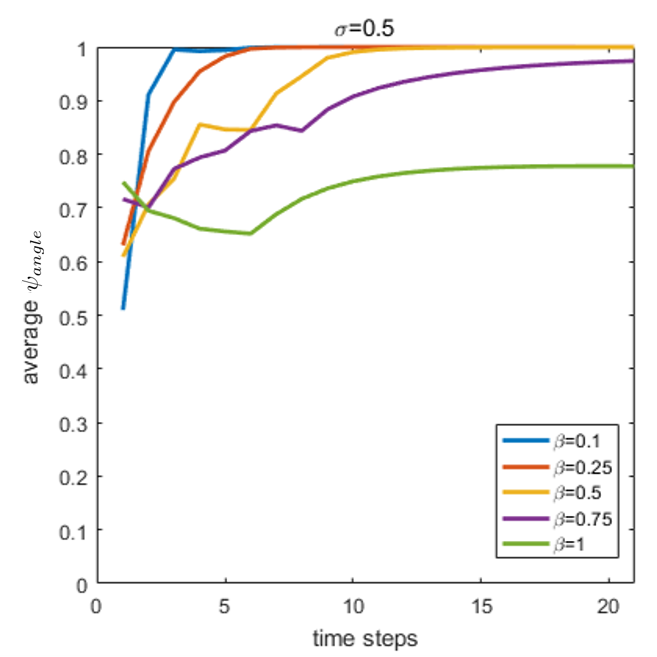
\includegraphics[width=0.48\textwidth]{figure/chapter_5/sigma0_5.png}}
  \subfigure[Case 2: $\sigma=1$]{\label{fig:sigma1}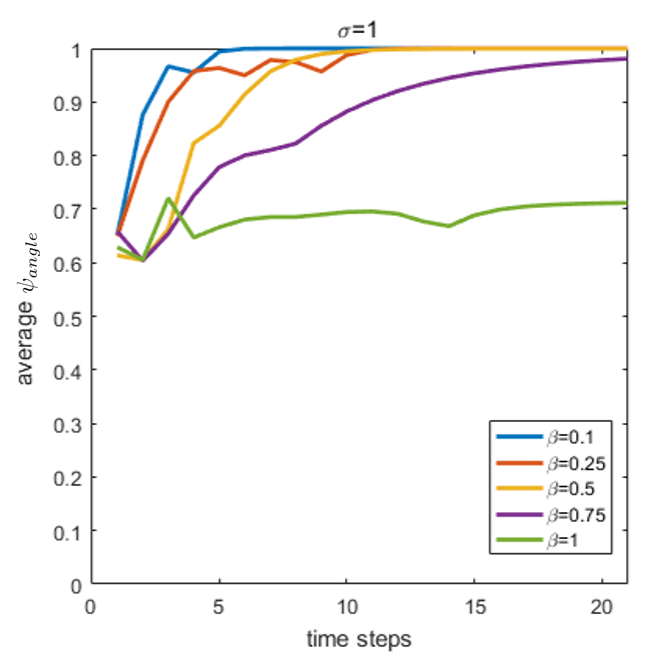
\includegraphics[width=0.48\textwidth]{figure/chapter_5/sigma1.png}}
  \quad
  \subfigure[Case 3: $\sigma>1$ with $\sigma=1.5$]{\label{fig:sigma1_5}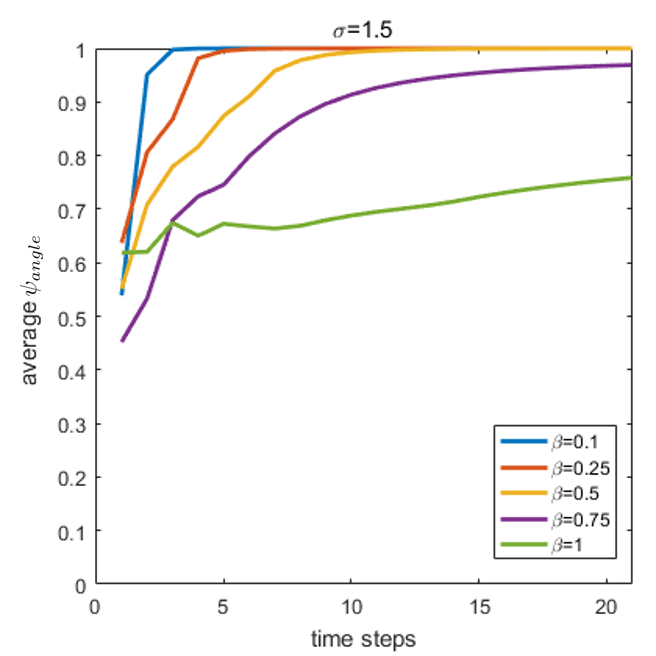
\includegraphics[width=0.48\textwidth]{figure/chapter_5/sigma1_5.png}}
  \caption{Averaged $\psi_{scal}$ of twenty simulations of two agents w.r.t various $\sigma, \beta$. The initial velocity are all randomized and nonzero.}\label{fig:sigma_beta}
\end{figure}

\begin{figure}[htb]
  \centering
  \subfigure[Multiple agents with fixed $\sigma, \beta$]{\label{fig:multiple}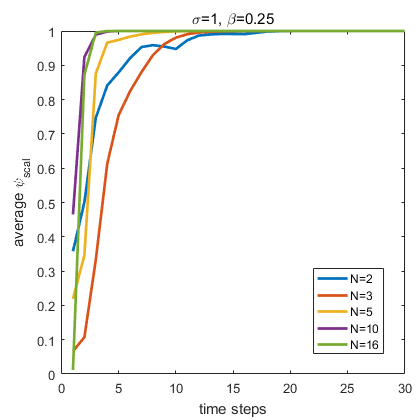
\includegraphics[width=0.48\textwidth]{figure/chapter_5/multiple.png}}
  \subfigure[Multiple agents with fixed $\sigma, \beta$]{\label{fig:distance}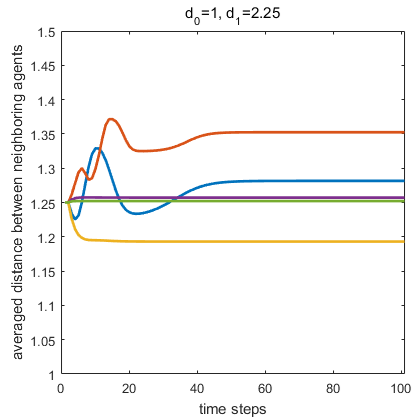
\includegraphics[width=0.48\textwidth]{figure/chapter_5/distance.png}}
  \caption{(a): Fixed $\sigma, \beta$ with various number of agents. The initial velocity are all randomized and nonzero. (b): Corresponding averaged distance between neighboring agents.}\label{fig:multiple_distance}
\end{figure}

We first simulate the flocking model with various $a_{ij}$ and control laws in Ch.~\ref{flocking} with 2, 3 and 4 agents respectively. The initial position are illustrated in Fig.\ref{fig:simulate_flocking} where only the most front agent has initial velocity pointing forward.
\begin{figure}[htb]
  \centering
  \subfigure[Two agents in a shape of straight line]{\label{fig:2_agents}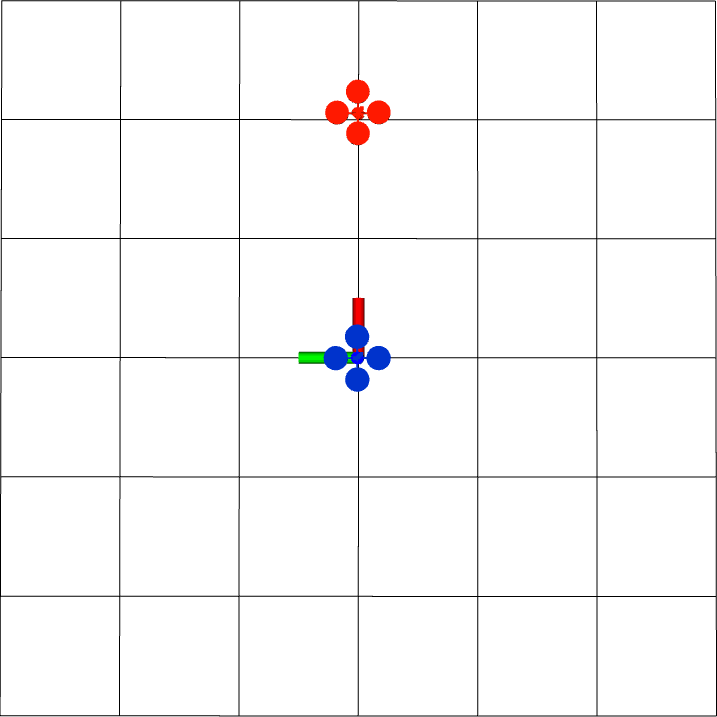
\includegraphics[width=0.48\textwidth]{figure/chapter_5/2_agent.png}}
  \subfigure[Three agents in a shape of equilateral triangle]{\label{fig:2_agents}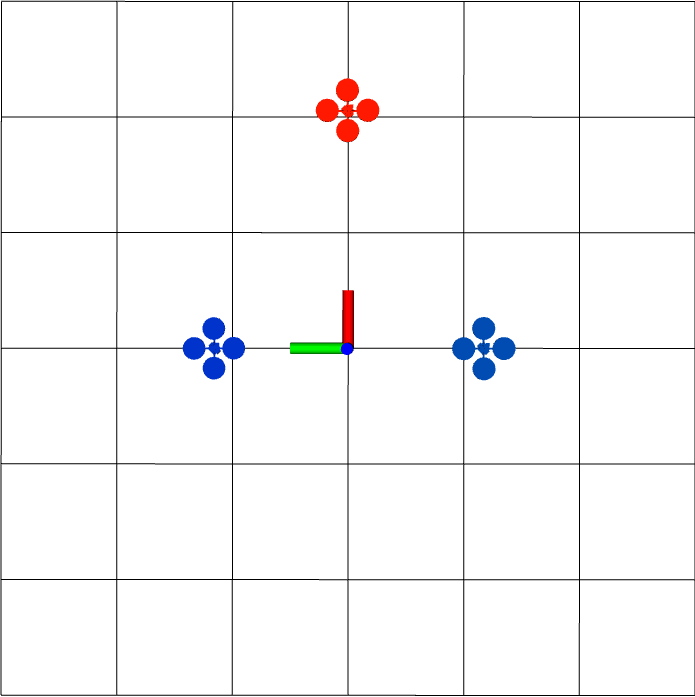
\includegraphics[width=0.48\textwidth]{figure/chapter_5/3_agent.png}}
  \quad
  \subfigure[Four agents in a shape of diamond]{\label{fig:2_agents}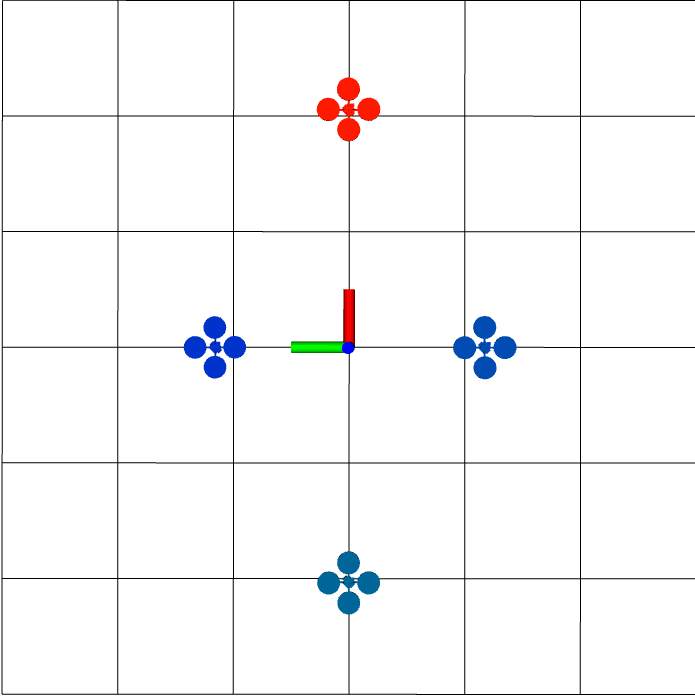
\includegraphics[width=0.48\textwidth]{figure/chapter_5/4_agent.png}}
  \caption{Simulations of multi-UAV flocking}\label{fig:simulate_flocking}
\end{figure}
